\chapter{Others}
\section{vimrc\ \small(gy)}
	\inputminted{vim}{Others/.vimrc}
\section{STL释放内存\ \small(Durandal)}
	\inputminted{cpp}{Others/stl_clear.cpp}
\section{开栈\ \small(Durandal)}
	\inputminted{cpp}{Others/rsp.cpp}
\section{O3\ \small(gy)}
	\inputminted{cpp}{Others/o3.cpp}
\section{读入优化\ \small(ct)}
    \inputminted{cpp}{Others/input_optimize.cpp}
\section{Java\ Template\ \small(gy)}
	\inputminted{java}{Others/Template.java}
\section{模拟退火\ \small(ct)}
	\inputminted{cpp}{Others/simulated_annealing.cpp}
\section{Simpson积分\ \small(gy)}
	\inputminted{cpp}{Others/simpson.cpp}
\section{Zeller\ Congruence\ \small(gy)}
	\inputminted{cpp}{Others/zeller_congruence.cpp}
\section{博弈论模型\ \small(gy)}
	\begin{itemize}
		\item Wythoff's game
			\\给定两堆石子,每次可以从任意一堆中取至少一个石子,或从两堆中取相同的至少一个石子,取走最后石子的胜
			\\先手胜当且仅当石子数满足:
			\\$\lfloor (b - a) \times \phi \rfloor=a, (a \leq b, \phi = \frac{\sqrt{5} + 1}{2})$
			\\先手胜对应的石子数构成两个序列:
			\\Lower Wythoff sequence: $a_n = \lfloor n \times \phi \rfloor$
			\\Upper Wythoff sequence: $b_n = \lfloor n \times \phi ^ 2 \rfloor$
		\item Fibonacci nim
			\\给定一堆石子,第一次可以取至少一个、少于石子总数数量的石子,之后每次可以取至少一个、不超过上次取石子数量两倍的石子,取走最后石子的胜
			\\先手胜当且仅当石子数为斐波那契数
		\item anti-SG
			\\决策集合为空的游戏者胜
			\\先手胜当且仅当满足以下任一条件
			\begin{itemize}[nosep]
				\item 所有单一游戏的$ SG $值都$ < 2 $且游戏的$ SG $值为$ 0 $
				\item 至少有一个单一游戏的$ SG $值$ \geq 2 $且游戏的$ SG $值不为$ 0 $
			\end{itemize}
	\end{itemize}
\section{积分表\ \small(integral-table.com)}
	\begin{multicols}{2}
		\tiny
\begin{equation*}
\int \frac{1}{a^2+x^2}dx = \frac{1}{a}\tan^{-1}\frac{x}{a}
\end{equation*}

\begin{equation*}
\int \frac{x}{a^2+x^2}dx = \frac{1}{2}\ln|a^2+x^2|
\end{equation*}

\begin{equation*}
\int \frac{x^2}{a^2+x^2}dx = x-a\tan^{-1}\frac{x}{a}
\end{equation*}

\begin{equation*}
\int \frac{x^3}{a^2+x^2}dx = \frac{1}{2}x^2-\frac{1}{2}a^2\ln|a^2+x^2|
\end{equation*}

\begin{equation*}
\int \frac{1}{ax^2+bx+c}dx = \frac{2}{\sqrt{4ac-b^2}}\tan^{-1}\frac{2ax+b}{\sqrt{4ac-b^2}}
\end{equation*}

\begin{equation*}
\int \frac{x}{ax^2+bx+c}dx = \frac{1}{2a}\ln|ax^2+bx+c| 
-\frac{b}{a\sqrt{4ac-b^2}}\tan^{-1}\frac{2ax+b}{\sqrt{4ac-b^2}}
\end{equation*}

\begin{equation*}
\int x\sqrt{x-a}\ dx =  
\frac{2 a}{3} \left({x-a}\right)^{3/2} +\frac{2 }{5}\left( {x-a}\right)^{5/2} 
\end{equation*}

\begin{equation*}
\int \frac{x}{\sqrt{x\pm a} } \ dx = \frac{2}{3}(x\mp 2a)\sqrt{x\pm a}
\end{equation*}

\begin{equation*}
\int \sqrt{\frac{x}{a-x}}\ dx =  -\sqrt{x(a-x)}
-a\tan^{-1}\frac{\sqrt{x(a-x)}}{x-a}
\end{equation*}

\begin{equation*}
\int \sqrt{\frac{x}{a+x}}\ dx =  \sqrt{x(a+x)} 
-a\ln \left ( \sqrt{x} + \sqrt{x+a}\right ) 
\end{equation*}

\begin{equation*}
\int x \sqrt{ax + b}\ dx =
\frac{2}{15 a^2}(-2b^2+abx + 3 a^2 x^2)
\sqrt{ax+b}
\end{equation*}

\begin{equation*}
\int \sqrt{x(ax+b)}\ dx =
 \frac{1}{4a^{3/2}}\left((2ax + b)\sqrt{ax(ax+b)} 
-b^2 \ln \left| a\sqrt{x} + \sqrt{a(ax+b)} \right| \right) 
\end{equation*}

\begin{equation*}
\int\sqrt{x^2 \pm a^2}\ dx = \frac{1}{2}x\sqrt{x^2\pm a^2} 
\pm\frac{1}{2}a^2 \ln \left | x + \sqrt{x^2\pm a^2} \right | 
\end{equation*}

\begin{equation*}
\int  \sqrt{a^2 - x^2}\ dx = \frac{1}{2} x \sqrt{a^2-x^2} 
+\frac{1}{2}a^2\tan^{-1}\frac{x}{\sqrt{a^2-x^2}}
\end{equation*}

\begin{equation*}
\int  x \sqrt{x^2 \pm a^2}\ dx= \frac{1}{3}\left ( x^2 \pm a^2 \right)^{3/2} 
\end{equation*}

\begin{equation*}
\int \frac{1}{\sqrt{x^2 \pm a^2}}\ dx = \ln \left | x + \sqrt{x^2 \pm a^2} \right | 
\end{equation*}

\begin{equation*}
\int \frac{1}{\sqrt{a^2 - x^2}}\ dx = \sin^{-1}\frac{x}{a} 
\end{equation*}

\begin{equation*}
\int \frac{x}{\sqrt{x^2\pm a^2}}\ dx = \sqrt{x^2 \pm a^2} 
\end{equation*}

\begin{equation*}
\int \frac{x}{\sqrt{a^2-x^2}}\ dx = -\sqrt{a^2-x^2} 
\end{equation*}

\begin{equation*}\label{eq:Russ}
\int \frac{x^2}{\sqrt{x^2 \pm a^2}}\ dx = \frac{1}{2}x\sqrt{x^2 \pm a^2}
\mp \frac{1}{2}a^2 \ln \left| x + \sqrt{x^2\pm a^2} \right | 
\end{equation*}

\begin{equation*}
\int\frac{1}{\sqrt{ax^2+bx+c}}\ dx=
\frac{1}{\sqrt{a}}\ln \left| 2ax+b + 2 \sqrt{a(ax^2+bx+c)} \right | 
\end{equation*}

\begin{equation*}\label{eq:Winokur2}
\int\frac{dx}{(a^2+x^2)^{3/2}}=\frac{x}{a^2\sqrt{a^2+x^2}}
\end{equation*}

\begin{equation*}
\int \sin^2 ax \cos bx\ dx = 
-\frac{\sin[(2a-b)x]}{4(2a-b)} 
+ \frac{\sin bx}{2b} 
- \frac{\sin[(2a+b)x]}{4(2a+b)}
\end{equation*}

\begin{equation*}
\int \cos^2 ax \sin bx\ dx = \frac{\cos[(2a-b)x]}{4(2a-b)} 
- \frac{\cos bx}{2b}
- \frac{\cos[(2a+b)x]}{4(2a+b)}
\end{equation*}

\begin{equation*}
\int \tan ax\ dx = -\frac{1}{a} \ln \cos ax 
\end{equation*}

\begin{equation*}
\int \tan^2 ax\ dx = -x + \frac{1}{a} \tan ax 
\end{equation*}

\begin{equation*}
\int \sec x \ dx = \ln | \sec x + \tan x | = 2 \tanh^{-1} \left (\tan \frac{x}{2} \right) 
\end{equation*}

\begin{equation*}
\int \sec^2 ax\ dx = \frac{1}{a} \tan ax 
\end{equation*}

\begin{equation*}
\int \csc x\ dx = \ln \left | \tan \frac{x}{2} \right|  = \ln | \csc x - \cot x| + C
\end{equation*}

\begin{equation*}
\int \csc^2 ax\ dx = -\frac{1}{a} \cot ax 
\end{equation*}

\begin{equation*}
\int \sec x \csc x \ dx = \ln | \tan x | 
\end{equation*}

\begin{equation*}
\int x \cos x \ dx = \cos x + x \sin x 
\end{equation*}

\begin{equation*}
\int x \sin x\ dx = -x \cos x + \sin x 
\end{equation*}

\begin{equation*}
\int x \cos^2 x \ dx = \frac{x^2}{4}+\frac{1}{8}\cos 2x + \frac{1}{4} x \sin 2x
\end{equation*}

\begin{equation*}
\int x \sin^2 x \ dx = \frac{x^2}{4}-\frac{1}{8}\cos 2x - \frac{1}{4} x \sin 2x
\end{equation*}
\small

	\end{multicols}
\section{STL\ Container\ Interface\ \small(cppreference.com)}
	\ifodd\thepage
		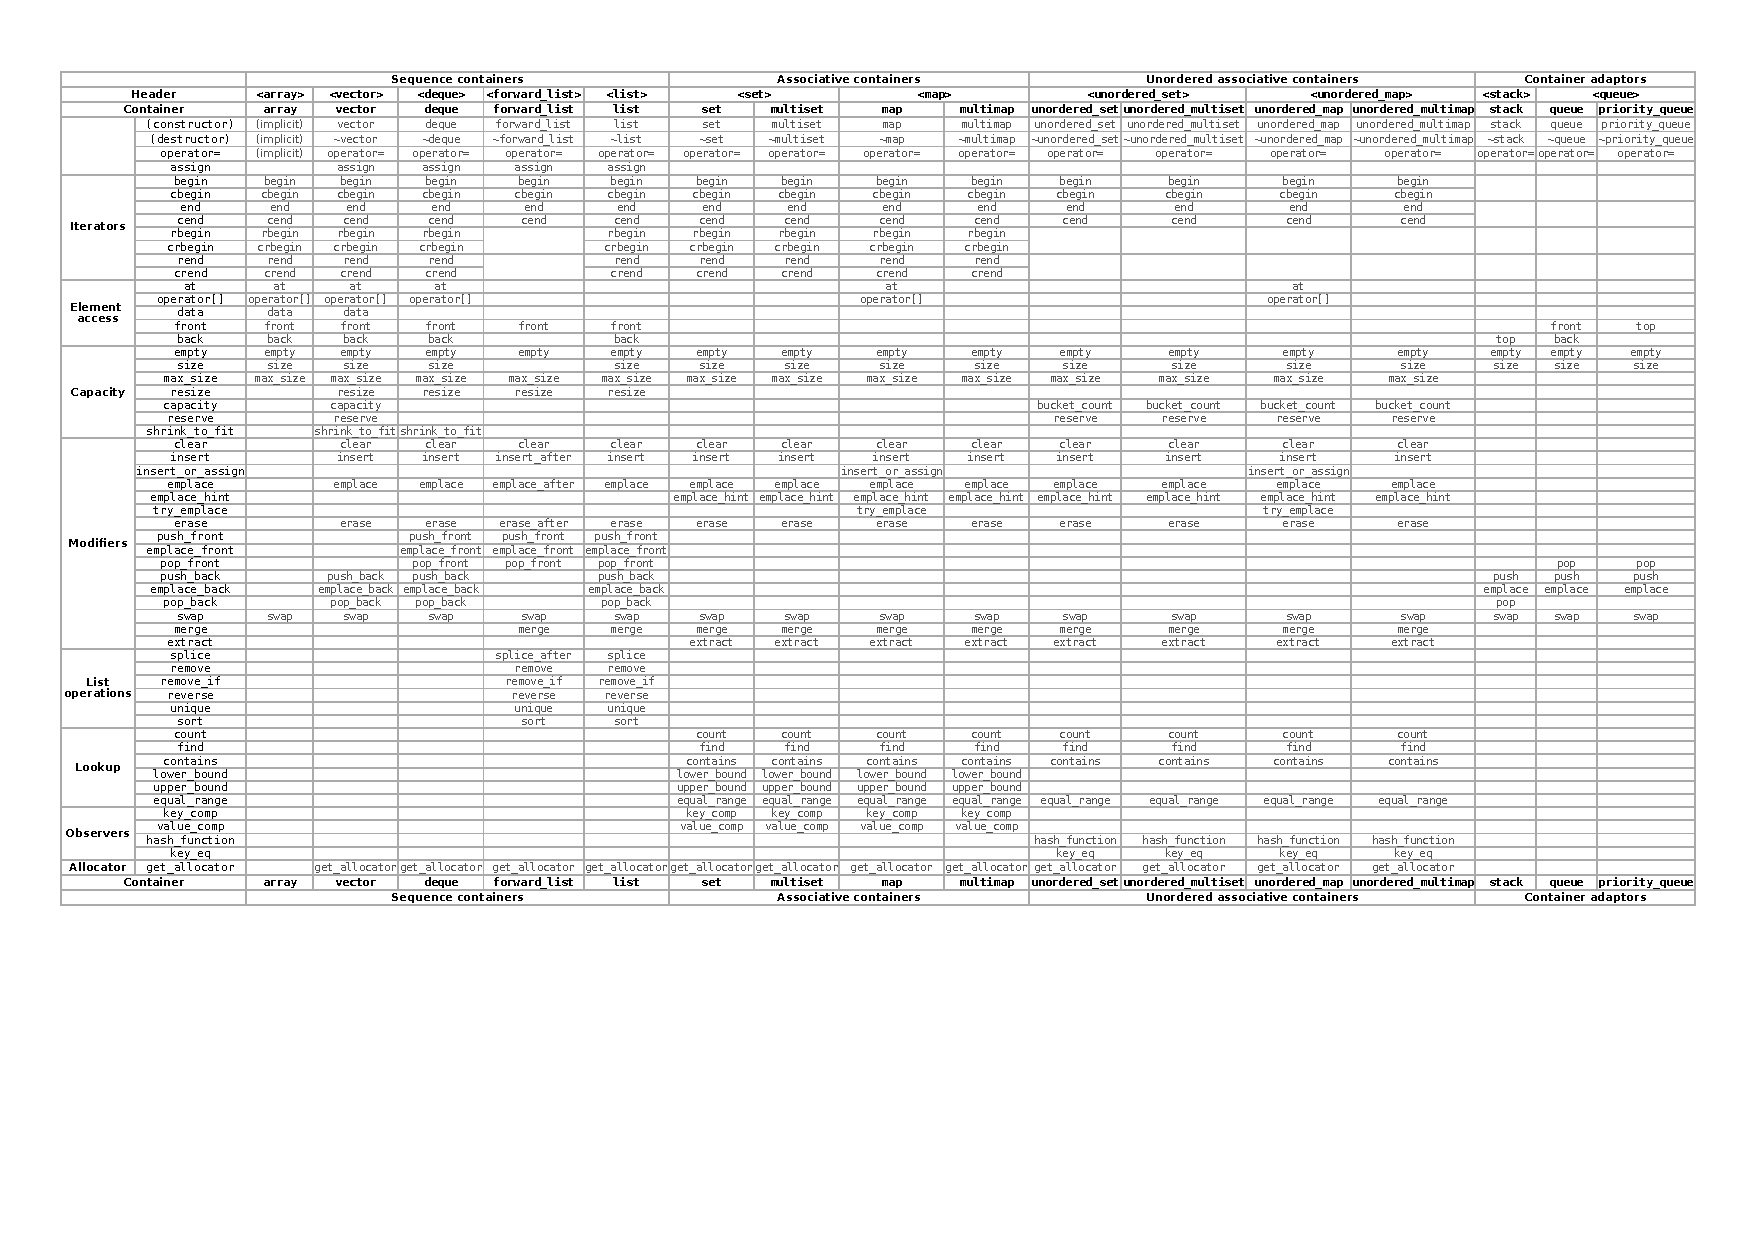
\includepdf[angle=270]{Others/stl.pdf}
	\else
		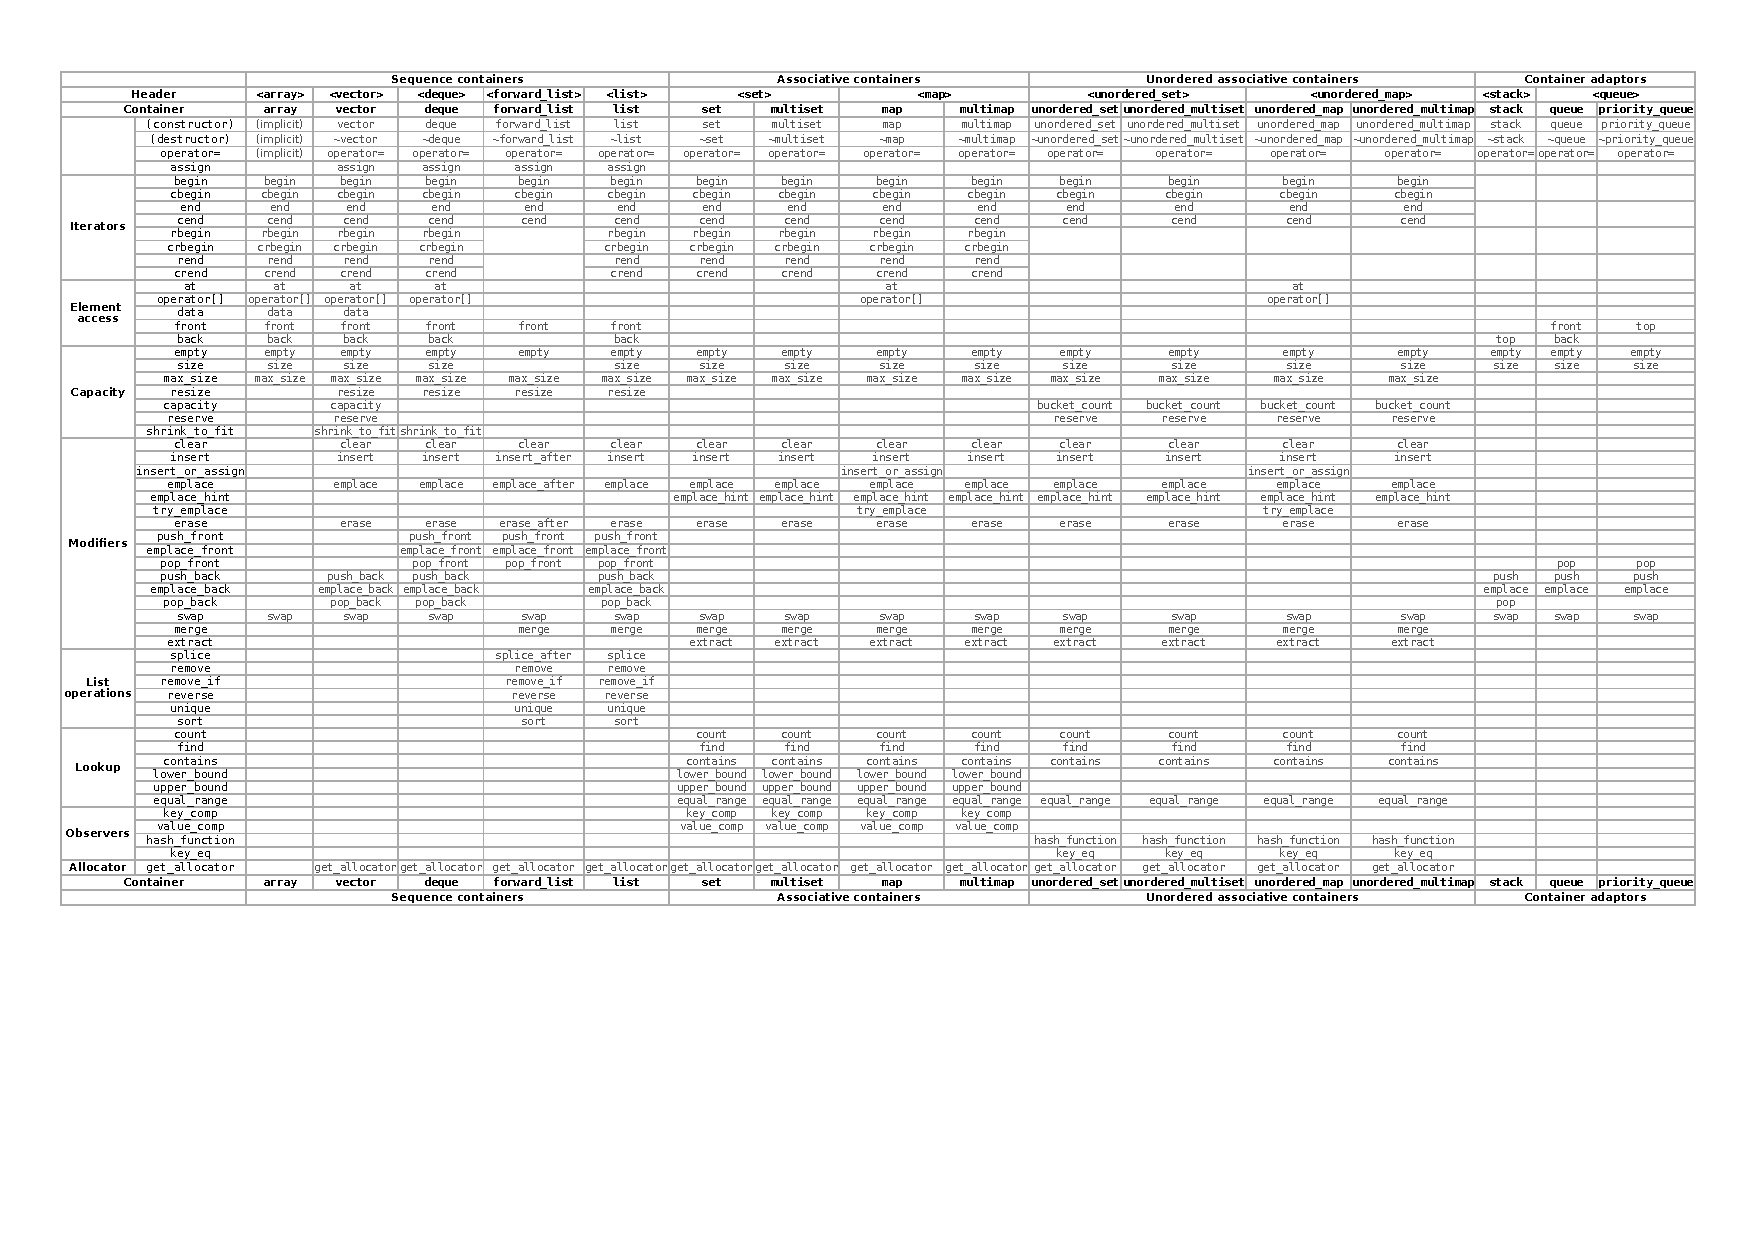
\includepdf[angle=90]{Others/stl.pdf}
	\fi
